\begin{frame}
	\begin{block} <1-> {Eigenschaften}
		\begin{itemize}
			\item <2-> Programmiersprache: Python
			\item <3-> Umsetzung mit Heap (Priority Queue)
			\item <4-> keine Speicherung der Farbstufen wie bei Dijkstra
				\begin{itemize}
					\item <5-> kürzerer und übersichtlicherer Code
				\end{itemize}
		\end{itemize}
	\end{block}	
\end{frame}


\begin{frame}
\frametitle{Kompletter Code}
	\centering
	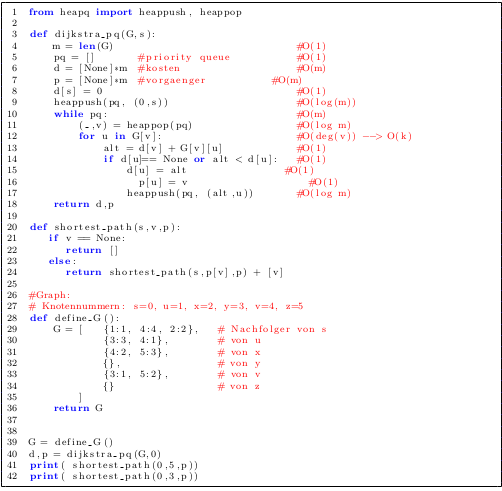
\includegraphics[scale=0.4]{./pictures/Impl.png}
\end{frame}


\begin{frame}
	\frametitle{Eingabe}
	\centering
	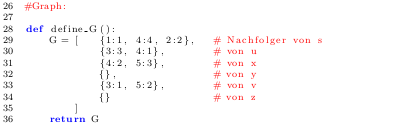
\includegraphics[scale=0.8]{./pictures/Eingabe.png}
\end{frame}


\begin{frame}
	\frametitle{Algorithmus-Initialisierung}
	\centering
	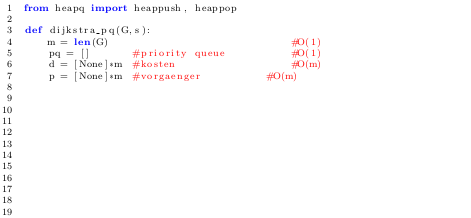
\includegraphics[scale=0.8]{./pictures/Init.png}
\end{frame}


\begin{frame}
	\frametitle{Algorithmus-Initialisierung}
	\centering
	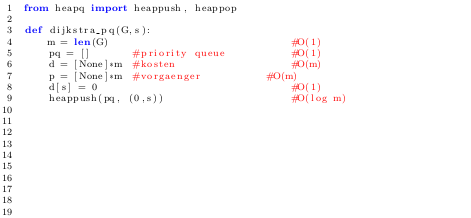
\includegraphics[scale=0.8]{./pictures/Startknoten.png}
\end{frame}


\begin{frame}
	\frametitle{Algorithmus-Erweitern}
	\centering
	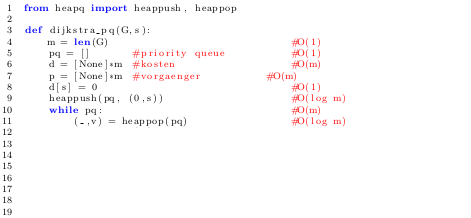
\includegraphics[scale=0.8]{./pictures/Knoten_entnehmen.png}
\end{frame}

\begin{frame}
	\frametitle{Algorithmus-Erweitern}
	\centering
	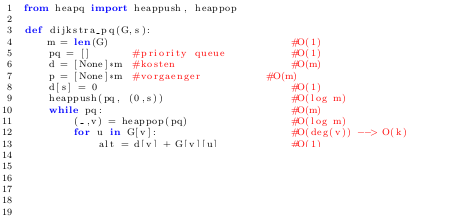
\includegraphics[scale=0.8]{./pictures/Pfad_berechnen.png}
\end{frame}

\begin{frame}
	\frametitle{Algorithmus-Aktualisieren}
	\centering
	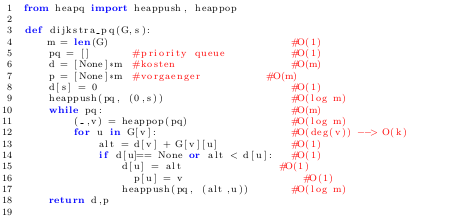
\includegraphics[scale=0.8]{./pictures/Relaxieren.png}
\end{frame}


\begin{frame}
	\begin{block} {Rekursives Bestimmen des Pfades}
		\vspace{3mm}
		\hspace{10mm}
		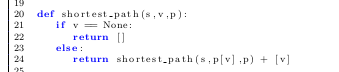
\includegraphics[scale=0.8]{./pictures/RekPfad.png}
	\end{block}
	\begin{block} {Aufruf}
	
		\hspace{11mm}
		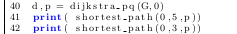
\includegraphics[scale=0.8]{./pictures/Aufruf.png}
	\end{block}
	
\end{frame}


			

